% !TeX TXS-program:compile = txs:///pdflatex/[--shell-escape]

\documentclass[10pt,  english, makeidx, a4paper, titlepage, oneside]{book}
\usepackage{babel}
\usepackage{fancyhdr}
\usepackage{makeidx}
\usepackage{titlesec}
\usepackage{listings}
\usepackage{booktabs}

\newenvironment{listato}{\footnotesize}{\normalsize }

%\pagestyle{empty}

\textwidth 15.5cm
\textheight 23cm
\topmargin -1cm
\oddsidemargin -0.5cm
\linespread{1.1}

\pagestyle{fancy}
\lhead{}
\chead{Example Report}
\lfoot{}
\cfoot{}
\rfoot{}
\rhead{\thepage}

\usepackage{graphicx}
\usepackage{amsmath}
\usepackage{amsfonts}
\usepackage{amsthm}
\usepackage{amssymb}
%\oddsidemargin -1.1cm
\usepackage{graphicx}
\usepackage{caption}
\usepackage{float}
\usepackage{amsmath}
\usepackage{amssymb}
\usepackage{amsfonts}
\usepackage{amsthm}
%\usepackage{subscript}
\usepackage{empheq}
\usepackage{verbatim}
\usepackage{fancyvrb}
\usepackage{hyperref}

% Code packages
\usepackage{listings}
\usepackage{minted}
\usepackage{tikz}
\usepackage{bytefield}
\usepackage{xparse}
\usepackage{etoolbox}

% For circuit diagrams
\usepackage[siunitx, RPvoltages]{circuitikz}
\usepackage{amsmath,amsbsy,amsfonts,amssymb}
\usepackage[per-mode=symbol]{siunitx}
\usepackage{steinmetz}
\usepackage[utf8]{inputenc}
\usepackage[edges]{forest}
%\usepackage[T1]{fontenc}


\definecolor{folderbg}{RGB}{124,166,198}
\definecolor{folderborder}{RGB}{110,144,169}

\def\Size{4pt}
\tikzset{
      folder/.pic={
        \filldraw[draw=folderborder,top color=folderbg!50,bottom color=folderbg]
          (-1.05*\Size,0.2\Size+5pt) rectangle ++(.75*\Size,-0.2\Size-5pt);  
        \filldraw[draw=folderborder,top color=folderbg!50,bottom color=folderbg]
          (-1.15*\Size,-\Size) rectangle (1.15*\Size,\Size);
      }
    }

\newcommand{\micro}{\ensuremath{\mu}}
\newcommand{\phasorName}[1]{ \ensuremath{ \boldsymbol{\hat #1} } }
\newcommand{\impedance}[1]{ \ensuremath{ \boldsymbol{#1} } }
\newcommand{\complexPol}[2]{\ensuremath{#1\phase{#2}}}
\newcommand{\complexPolDeg}[2]{\ensuremath{#1\phase{#2\degree}}}

% new units
\DeclareSIUnit{\Vef}{\volt_{ef}} % volt eficaz
\DeclareSIUnit{\Vrms}{\volt_{rms}} % volt RMS
\DeclareSIUnit{\Vpp}{\volt_{pp}} % volt peak-to-peak

\DeclareSIUnit{\Aef}{\ampere_{ef}} % ampere eficaz
\DeclareSIUnit{\Arms}{\ampere_{rms}} % ampere rms
\DeclareSIUnit{\App}{\ampere_{pp}} % ampere peak-to-peak

% logic Commands
\newcommand{\NOT}[1]{\ensuremath{\overline{\mbox{\ensuremath{#1}}}}}
\newcommand{\AND}{\ensuremath{\cdot}}
\newcommand{\OR}{\ensuremath{+}}
\newcommand{\XOR}{\ensuremath{\oplus}}
\newcommand{\XNOR}{\ensuremath{\odot}}

\newtoggle{newarg}
\toggletrue{newarg}
\newcounter{bitfieldsize}
\usetikzlibrary{positioning}
\usetikzlibrary{decorations.pathreplacing}

\newcommand\mybitbox[1] {% <- here
    \iftoggle{newarg}{% <- here
        \setcounter{bitfieldsize}{ #1 }% <- here
        \togglefalse{newarg}% <- here
    }{% <- here
        \bitbox{\value{bitfieldsize}}{#1}% <- here
        \toggletrue{newarg}% <- here
    }}

\NewDocumentCommand\bitboxlist {  >{\SplitList{;}}m} {% <- here
    \ProcessList{#1}{\mybitbox}}

\newcounter{instsize}
\NewDocumentCommand\mybytefield{m >{\SplitList{;}}m} {% <- here
    \setcounter{instsize}{#1 - 1 }% <- here
    \begin{figure}[htbp]
        \begin{center}
            \begin{bytefield}[endianness=big,bitwidth=1em]{#1}
                \bitheader{0-\value{instsize}} \\
                \ProcessList{#2}{\bitboxlist}% <- here
            \end{bytefield}
        \end{center}
    \end{figure}}

\newcommand\staticbitbox[4] {% <- here
    \bitbox{#1}{#2} \bitbox{#3}{#4}}


\newcommand\MemoryLayout[1]{
  \begin{tikzpicture}[scale=0.3]
     \draw[thick](0,0)--++(0,3)node[above]{$0$};
     \foreach \pt/\col/\lab [remember=\pt as \tp (initially 0)] in {#1} {
       \foreach \a in {\tp,...,\pt-1} {
          \draw[fill=\col](-\a,0) rectangle ++(-1,2);
       }
       \draw[thick](-\pt,0)--++(0,3)node[above]{$\pt$};
       \if\lab\relax\relax\else
         \draw[thick,decorate, decoration={brace,amplitude=4mm}]
            (-\tp,-0.2)--node[below=4mm]{\lab} (-\pt,-0.2);
       \fi
     }
  \end{tikzpicture}
}

\NewDocumentCommand{\codeword}{v}{%
\texttt{\textcolor{blue}{#1}}%
}



\newcommand\memsection[4]{
\bytefieldsetup{bitheight=#3\baselineskip}    % define the height of the memsection
\bitbox[]{10}{
\texttt{#1}     % print end address
\\ \vspace{#3\baselineskip} \vspace{-2\baselineskip} \vspace{-#3pt} % do some spacing
\texttt{#2} % print start address
}
\bitbox{16}{#4} % print box with caption
}

\lstdefinelanguage{VHDL}{morekeywords={library,use,all,entity,generic, is,port,in,out,end,architecture,of,begin,and,if,then,else,elsif,process},morecomment=[l]--}

\lstdefinestyle{vhdl}{language = VHDL, basicstyle = \ttfamily, keywordstyle = \color{keyword}\bfseries, commentstyle = \color{comment}}

\titleformat{\chapter}[display]
{\normalfont\Large\filcenter\sffamily}
{\titlerule[0.5pt]%
\vspace{1pt}
\titlerule
\vspace{1pc}
\LARGE\MakeUppercase{\chaptertitlename} \thechapter
}
{1pc}
{\titlerule
\vspace{1pc}
\Huge}

\makeindex

\begin{document}

% TEMPLATE: Insert logo for the presentation
\frontmatter
\begin{titlepage}
\vspace{0cm}
\centerline{
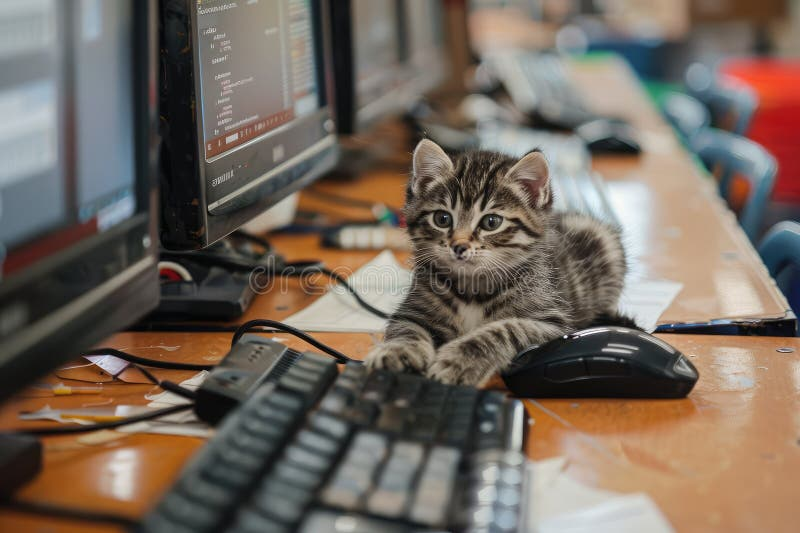
\includegraphics[width=0.6\textwidth]{chapters/figures/cat.png}} 
\vspace{0.5cm}
\centerline{\huge\sf Example Title}
\vspace{1cm}
\centerline{\Huge\sf More Title}
\bigskip
\centerline{\huge\sf MORE TITLE}
\vspace{1cm}
\centerline{\Large Master degree in more title}
\centerline{\Large Academic Year title/title}
\vspace{2.5cm}
%%%%%%%%%%%%%%%%%%%%%%%%%%%%%%%%%%%%%%%%%%%%%%%%%%%%%%
%
{\large Referents:}

Prof. Mario Rossi

Prof. Mario Rossi

Prof. Mario Rossi 

Prof. Mario Rossi

\bigskip
\vspace{1cm}
%
%%%%%%%%%%%%%%%%%%%%%%%%%%%%%%%%%%%%%%%%%%%%%%%%%%%%%%
%
{\large Authors:}
% \bigskip
%
%%%%%%%%%%%%%%%%%%%%%%%%%%%%%%%%%%%%%%%%%%%%%%%%%%%%%%
% AUTHORS

Mario Rossi

Mario Rossi

Mario Rossi

Mario Rossi

Mario Rossi

%
%%%%%%%%%%%%%%%%%%%%%%%%%%%%%%%%%%%%%%%%%%%%%%%%%%%%%%
\begin{center}
    {\large \today}
\end{center}
\end{titlepage}

\chapter{Abstract}\label{Abstract}

\tableofcontents

\mainmatter
%%%%%%%%%%%%%%%%%%%%%%%%%%%%%%%%%%%%%%%%%%%%%%%%%%%%%%
%    
%
\chapter{Introduction}

\section{Examples}

Example \href{https://www.lipsum.com/}{Link}

\subsection{Example subsection}

Unordered list:
\begin{itemize}
    \item Item 1 
    \item Item 2 
    \item Item 3 
    \item Item 4 
\end{itemize}

\begin{figure}[ht]
    \centering
    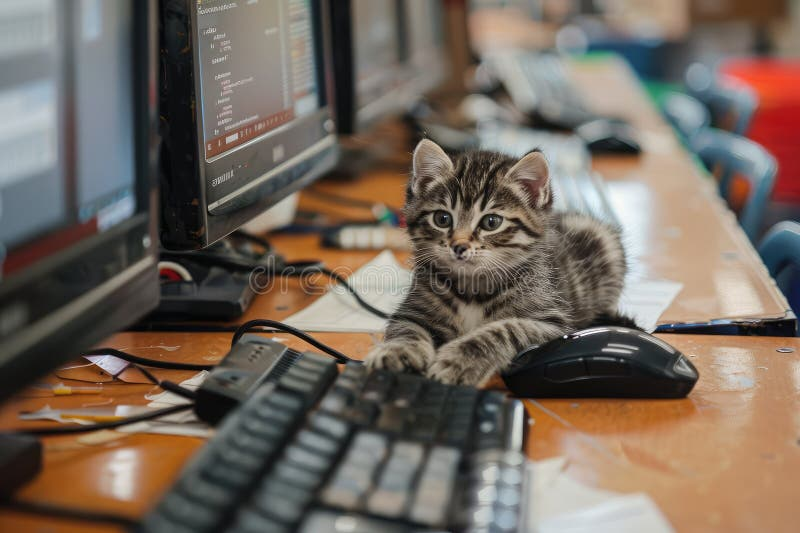
\includegraphics[width=0.6\textwidth]{chapters/figures/cat.png}
    \caption{Example image}
    \label{fig:example_image}
\end{figure}

This is an example for a folder structure: 
|
\begin{forest}
    for tree={
        font=\ttfamily,
        grow'=0,
        child anchor=west,
        parent anchor=south,
        anchor=west,
        calign=first,
        inner xsep=7pt,
        edge path={
          \noexpand\path [draw, \forestoption{edge}]
          (!u.south west) +(7.5pt,0) |- (.child anchor) pic {folder} \forestoption{edge label};
        },
        % style file node 
        file/.style={edge path={\noexpand\path [draw, \forestoption{edge}]
          (!u.south west) +(7.5pt,0) |- (.child anchor) \forestoption{edge label};},
          inner xsep=2pt,font=\small\ttfamily
                     },
        before typesetting nodes={
          if n=1
            {insert before={[,phantom]}}
            {}
        },
        fit=band,
        before computing xy={l=15pt},
      }  
  [Main Folder
    [Fodlder 1
      [Subfolder 1
        [SubSubfolder 1
            [File 1.c - Example 1, file]
            [File 2.c - Example 2, file]
        ]
        [SubSubfolder 3
            [File 3.c - Example 3, file]
        ]
      ]
      [Folder 2
        [Subfolder 1]
      ]
    ]
  ]
\end{forest}


\input{./chapters/chap2}
% \input{./chapters/chap3}
% \input{./chapters/chap4}
% \input{./chapters/chap5}
% \input{./chapters/chap6}
% \input{./chapters/chap_name}
%
%%%%%%%%%%%%%%%%%%%%%%%%%%%%%%%%%%%%%%%%%%%%%%%%%%%%%%
%    
%
\appendix
%%% Appendix A
\chapter{Code Section}\label{Code_Section}

\section{Code 1}\label{Code_1}
	\subsection{File 1}
	This is a file code example:
	\inputminted[breaklines]{c}{./appendices/files/example.c}
	
	This is a block code example:

	\begin{minted}{c}
#include <stdio.h>

int main() {
	printf("Hello, World!\n");
	return 0;
}
	\end{minted}

this is an inline code example: \mintinline{c}|printf("Hello, World!\n");|
% \input{./appendices/appendix2}
%
%%%%%%%%%%%%%%%%%%%%%%%%%%%%%%%%%%%%%%%%%%%%%%%%%%%%%%

\end{document}